\documentclass[12pt,a4paper]{article}

\usepackage[T2A]{fontenc}
\usepackage[utf8]{inputenc}
\usepackage[russian]{babel}
\usepackage{amsmath,amssymb}
\usepackage{array}
\usepackage{booktabs}
\usepackage{geometry}
\usepackage{graphicx}
\usepackage{float}
\usepackage{listings}
\usepackage{caption}
\usepackage{enumitem}
\usepackage{indentfirst}
\usepackage{personal_data}
\usepackage{hhline}

\geometry{left=25mm,right=20mm,top=20mm,bottom=20mm}
\setlength{\parindent}{1.25cm}
\setlength{\parskip}{0.3em}

\lstset{
    basicstyle=\ttfamily\small,
    columns=fullflexible,
    frame=single,
    breaklines=true,
    keepspaces=true
}

\begin{document}

\begin{titlepage}
\center 

\normalsize \textbf{Липецкий государственный технический университет}\\

\vspace{1 cm}

\normalsize Институт компьютерных наук\\
\normalsize Кафедра прикладной математики и системного анализа\\

\vspace{6 cm}

\normalsize 	Отчет по лабораторной работе № \nomer_lr\\
по дисциплине <<\diszip >> \\
на тему <<\thema >>
\vspace{1 cm}


\vspace*{3 cm}

\normalsize
\begin{tabular}{b{4.75cm} p{1cm} c p{1cm} c}
Студент  	&   &  &  &  \student \\ \hhline{~~-~-} 

 	&  & \footnotesize \hspace{0.5cm} подпись, дата	\hspace{0.5cm} &  & \footnotesize  фамилия, инициалы \\ [-0.25cm]
Группа \underline{\group}  	&   &  &  &  \\ [0.4cm]
Руководитель  	&   &  &  &  \\
\centering{\dz}	&   &  &  & \dozent \\ \hhline{-~-~-} 
\footnotesize учёная степень, учёное звание	 	&  	& \footnotesize \hspace{0.5cm} подпись, дата	\hspace{0.5cm} &  & \footnotesize  фамилия, инициалы \\

 
\end{tabular} 



\vspace*{5cm}
\normalsize
\centering Липецк 2026 г.

\end{titlepage}

%\tableofcontents
\newpage

\section{Задание}
Разработать программное обеспечение для построения интерполяционных многочленов Лагранжа и Ньютона на основе произвольно заданной табличной функции. Рассчитать значение функции в заданной пользователем точке $x^*$ на основе построенных интерполяционных многочленов, а так-же при помощи схемы Эйткена.

Предусмотреть вывод интерполяционных многочленов Лагранжа и Ньютона в изначальном и упрощенном виде (по убыванию степеней), а также вывод результатов вычислений разделенных разностей для многочлена Ньютона и промежуточных значений многочленов Лагранжа в схеме Эйткена. Показать значение в точке $x^*$, полученное по схеме Эйткена и при подстановке в каж-дый из интерполяционных многочленов.

Сравнить результаты, полученные разными способами.

Организовать обработку исключений:
\begin{enumerate}
    \item ввод некорректного символа, значения;
    \item точка $x^*$ находится вне отрезка интерполяции;
    \item узлы не упорядочены по возрастанию.
\end{enumerate}

\section{Теоретические сведения}

\subsection{Интерполяционный многочлен Лагранжа. Схема Эйткена}

Рассматриваются многочлены
\[
\varphi(x)=\sum_{i=0}^{n}a_ix^i
\]
с базисными функциями
\[
1,x,x^2,\ldots,x^n.
\]
Тогда
\[
|\Phi|=
\begin{vmatrix}
1 & x_0 & \ldots & x_0^n\\
1 & x_1 & \ldots & x_1^n\\
\vdots & \vdots & & \vdots\\
1 & x_n & \ldots & x_n^n
\end{vmatrix}
=\prod_{i>j}(x_i-x_j).
\]

Для выполнения условий
\[
\Phi_i(x_j)=\delta_{ij}
\]
фундаментальные многочлены имеют вид
\[
\Phi_i(x)=c_i(x-x_0)\ldots(x-x_{i-1})(x-x_{i+1})\ldots(x-x_n),
\]
откуда $\Phi_i(x_j)=0$ при $i\ne j$. Из условия нормировки
\[
\Phi_i(x_i)=c_i(x_i-x_0)\ldots(x_i-x_{i-1})(x_i-x_{i+1})\ldots(x_i-x_n)=1.
\]

Следовательно,
\begin{equation}
\Phi_i(x)=
\frac{(x-x_0)\ldots(x-x_{i-1})(x-x_{i+1})\ldots(x-x_n)}
{(x_i-x_0)\ldots(x_i-x_{i-1})(x_i-x_{i+1})\ldots(x_i-x_n)}
=
\frac{\prod\limits_{\substack{k=0\\k\ne i}}^{n}(x-x_k)}
{\prod\limits_{\substack{k=0\\k\ne i}}^{n}(x_i-x_k)}.
\end{equation}
Это фундаментальные многочлены Лагранжа.

Интерполяционный многочлен Лагранжа:
\begin{equation}
\varphi(x)=L_n(x)=
\sum_{i=0}^{n}f_i
\frac{\prod\limits_{\substack{k=0\\k\ne i}}^{n}(x-x_k)}
{\prod\limits_{\substack{k=0\\k\ne i}}^{n}(x_i-x_k)}.
\end{equation}

Узловой многочлен:
\[
\omega(x)=(x-x_0)(x-x_1)\ldots(x-x_n)=\prod_{k=0}^{n}(x-x_k).
\]
Тогда многочлен Лагранжа можно записать в виде
\[
L_n(x)=
\sum_{i=0}^{n}
\frac{f_i\omega(x)}{(x-x_i)\omega'(x_i)}
=
\omega(x)
\sum_{i=0}^{n}
\frac{f_i}{(x-x_i)\omega'(x_i)}.
\]

При больших $n$ вычисления громоздки. Вычисления значений многочленов Лагранжа различных порядков в заданной точке $x$ удобно проводить рекуррентным образом по интерполяционной схеме Эйткена:
\[
L_i(x)=f_i,
\]
\[
L_{0,1}=
\frac{1}{x_1-x_0}
\begin{vmatrix}
x-x_0 & L_0\\
x-x_1 & L_1
\end{vmatrix}
\]
--- интерполяционный многочлен Лагранжа 1-го порядка;
\[
L_{1,2}=
\frac{1}{x_2-x_1}
\begin{vmatrix}
x-x_1 & L_1\\
x-x_2 & L_2
\end{vmatrix}.
\]

Далее:
\[
L_{0,1,2}=
\frac{1}{x_2-x_0}
\begin{vmatrix}
x-x_0 & L_{0,1}\\
x-x_2 & L_{1,2}
\end{vmatrix}
\]
--- интерполяционные многочлены 2-го порядка;
\[
L_{0,1,\ldots,i}=
\frac{1}{x_i-x_0}
\begin{vmatrix}
x-x_0 & L_{0,1,\ldots,i-1}\\
x-x_i & L_{1,2,\ldots,i}
\end{vmatrix}
\]
--- интерполяционные многочлены порядка $i$.

\subsection{Интерполяционный многочлен Ньютона}

Разделённые разности 1-го порядка:
\[
f(x_0,x_1)=\frac{f_1-f_0}{x_1-x_0},\qquad
f(x_1,x_2)=\frac{f_2-f_1}{x_2-x_1},\qquad
f(x_{n-1},x_n)=\frac{f_n-f_{n-1}}{x_n-x_{n-1}}.
\]

Разделённые разности 2-го порядка:
\[
f(x_0,x_1,x_2)=\frac{f(x_1,x_2)-f(x_0,x_1)}{x_2-x_0},
\]
\[
f(x_{n-2},x_{n-1},x_n)=
\frac{f(x_{n-1},x_n)-f(x_{n-2},x_{n-1})}{x_n-x_{n-2}}.
\]

Разделённые разности $(k+1)$-го порядка:
\[
f(x_{i-1},x_i,\ldots,x_{i+k})=
\frac{f(x_i,x_{i+1},\ldots,x_{i+k})-f(x_{i-1},x_i,\ldots,x_{i+k-1})}
{x_{i+k}-x_{i-1}}.
\]

Заметим, что
\[
f(x_i,x_{i+1},\ldots,x_{i+k})=
\sum_{j=0}^{k}
\frac{f(x_{i+j})}
{(x_{i+j}-x_i)\ldots(x_{i+j}-x_{i+j-1})(x_{i+j}-x_{i+j+1})\ldots(x_{i+j}-x_{i+k})}.
\]

Пусть $x$ --- произвольная фиксированная точка. Тогда
\[
f(x,x_0)=\frac{f(x_0)-f(x)}{x_0-x},
\]
\[
f(x)=f(x_0)+f(x,x_0)(x-x_0).
\]

Для разделённой разности 2-го порядка:
\[
f(x,x_0,x_1)=\frac{f(x_0,x_1)-f(x,x_0)}{x_1-x},
\]
\[
f(x,x_0)=f(x_0,x_1)+f(x,x_0,x_1)(x-x_1).
\]

Интерполяционная формула Ньютона для неравноотстоящих узлов:
\[
f(x)\approx P_n(x)=
f(x_0)+f(x_0,x_1)(x-x_0)+
f(x_0,x_1,x_2)(x-x_0)(x-x_1)+\ldots
\]
\[
\ldots+
f(x_0,x_1,\ldots,x_n)(x-x_0)(x-x_1)\ldots(x-x_{n-1}).
\]

Остаточный член:
\[
R_n(x)=f(x)-P_n(x)=f(x,x_0,x_1,\ldots,x_n)\omega(x).
\]

Вычисления разделённых разностей удобно представлять в виде таблицы.

% =================================================
% 2. Листинг
% =================================================

\section{Листинг программы}

\subsection{Реализация метода Лагранжа}

\begin{lstlisting}
#include <vector>

class Lagrange {
    std::vector<double>polynom;
    std::vector<double>x,y;
    int n;
public:
    Lagrange(std::vector<double>n_x, std::vector<double>n_y) : x(n_x), y(n_y), n(x.size()) {
        polynom.resize(n, 0);
        buildPolynom();
    }

    void buildPolynom() {
        for (int i = 0; i < n; i++) {
            if (y[i] == 0) continue;

            double mul = y[i];
            for (int j = 0; j < n; j++) {
                if (j != i) mul /= (x[i] - x[j]);
            }

            std::vector<double>cur(2);
            cur[1] = 1;
            cur[0] = -(i == 0 ? x[1] : x[0]);
            for (int j = 0; j < n; j++) {
                if (i == j) continue;
                if (i == 0 && j == 1) continue;
                if (i >= 1 && j == 0) continue;
                std::vector<double>next(cur.size() + 1, 0);
                next[0] = -1 * cur[0] * x[j];
                for (int k = 1; k < next.size() - 1; k++) {
                    next[k] = cur[k - 1] - x[j] * cur[k];
                }
                next[next.size() - 1] = cur[cur.size() - 1];
                cur = next;
            }
            for (int j = 0; j < n; j++) {
                polynom[j] += cur[j] * mul;
            }
        }
    }

    std::vector<double> getPolynom() {
        return polynom;
    }

    double getValueInPoint(double find_x) {
        double value = 0;
        for (int i = n - 1; i >= 0; i--) {
            value = value * find_x + polynom[i];
        }
        return value;
    }
};
\end{lstlisting}

\subsection{Реализация метода Ньютона}

\begin{lstlisting}
#include <vector>
#include <iostream>

class Newton {
    std::vector<double>polynom;
    std::vector<double>x,y;
    int n;
    std::vector<std::vector<double>>rr;

public:
    Newton(std::vector<double>n_x, std::vector<double>n_y) : x(n_x), y(n_y), n(x.size()) {
        polynom.resize(n, 0);
        buildRR();
        buildPolynom();
    }

    void buildRR() {
        rr.resize(n);
        for (int i = 0; i < n; i++) rr[0].push_back(y[i]);
        for (int i = 1; i < n; i++) {
            for (int j = 0; j < n - i; j++) {
                rr[i].push_back((rr[i - 1][j + 1] - rr[i - 1][j]) / (x[i + j] - x[j]));
            }
        }
    }

    void buildPolynom() {
        polynom[0] = y[0];
        
        for (int i = 1; i < n; i++) {
            std::vector<double>cur(2);
            cur[0] = -x[0];
            cur[1] = 1;
            for (int j = 1; j < i; j++) {
                std::vector<double>next(cur.size() + 1, 0);
                next[0] = -1 * cur[0] * x[j];
                for (int k = 1; k < next.size() - 1; k++) {
                    next[k] = cur[k - 1] - x[j] * cur[k];
                }
                next[next.size() - 1] = cur[cur.size() - 1];
                cur = next;
            }

            for (int j = 0; j < cur.size(); j++) {
                polynom[j] += cur[j] * rr[i][0];
            }
        }
    }

    std::vector<double> getPolynom() {
        return polynom;
    }

    double getValueInPoint(double find_x) {
        double value = 0;
        for (int i = n - 1; i >= 0; i--) {
            value = value * find_x + polynom[i];
        }
        return value;
    }

    std::vector<std::vector<double>> getRR() {
        return rr;
    }
};
\end{lstlisting}

\subsection{Реализация метода Эйткена}

\begin{lstlisting}
#include <vector>

class Aitken {
    std::vector<double>x,y;
    int n;

public:
    Aitken(std::vector<double>n_x, std::vector<double>n_y) : x(n_x), y(n_y), n(x.size()) {}

    double getValueInPoint(double find_x) {
        std::vector<double>polynoms = y;

        for (int i = 1; i < n; i++) {
            std::vector<double>next(n - i);
            for (int j = 0; j < n - i; j++) {
                next[j] = (polynoms[j + 1] * (find_x - x[j])
                           - polynoms[j] * (find_x - x[i + j]))
                           / (x[i + j] - x[j]);
            }
            polynoms = next;
        }
        return polynoms[0];
    }

    std::vector<std::vector<double>> buildTable(double findX) {
        const int n = static_cast<int>(x.size());
        std::vector<std::vector<double>> table(n);

        table[0] = y;

        for (int k = 1; k < n; ++k) {
            table[k].resize(n - k);

            for (int j = 0; j < n - k; ++j) {
                table[k][j] =
                    (table[k - 1][j + 1] * (findX - x[j])
                    - table[k - 1][j] * (findX - x[j + k]))
                    / (x[j + k] - x[j]);
            }
        }

        return table;
    }
};
\end{lstlisting}

\subsection{Реализация вывода полинома}

\begin{lstlisting}
string polynomialFromCoefficients(const vector<double>& c) {
    string result;
    const double EPS = 1e-6;

    for (int i = static_cast<int>(c.size()) - 1; i >= 0; --i) {
        if (std::abs(c[i]) < EPS) continue;

        double a = c[i];
        bool negative = a < 0;
        double absA = std::abs(a);

        if (result.empty()) {
            if (negative) result += "-";
        } else {
            result += negative ? " - " : " + ";
        }

        if (i == 0) {
            result += num(absA);
        } else {
            if (std::abs(absA - 1.0) > EPS) {
                result += num(absA) + "*";
            }
            result += variablePower(i);
        }
    }

    return result.empty() ? "0" : result;
}
\end{lstlisting}


\section{Пример работы}

\begin{figure}[H]
    \centering
    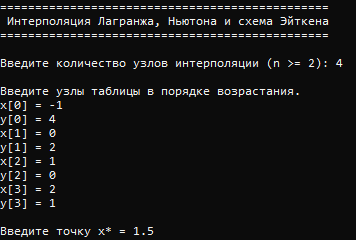
\includegraphics[scale=1]{input.png}
    \caption{Ввод}
    \label{fig:success}
\end{figure}

\begin{figure}[H]
    \centering
    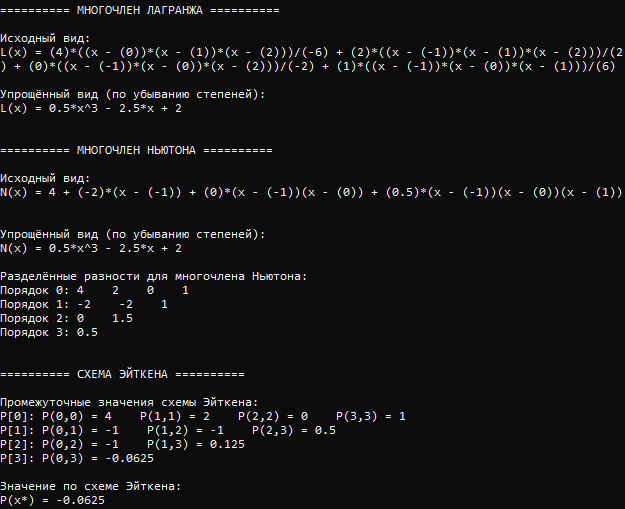
\includegraphics[scale=1]{methods.png}
    \caption{Вывод трёх методов}
    \label{fig:success}
\end{figure}

\begin{figure}[H]
    \centering
    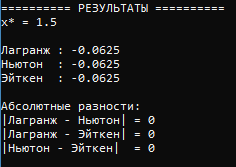
\includegraphics[scale=1]{result.png}
    \caption{Результат работы программы}
    \label{fig:success}
\end{figure}

\begin{figure}[H]
    \centering
    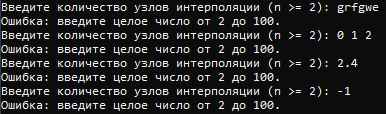
\includegraphics[scale=1]{error_1.png}
    \caption{Обработка ошибок при вводе кол-ва точек}
    \label{fig:success}
\end{figure}

\begin{figure}[H]
    \centering
    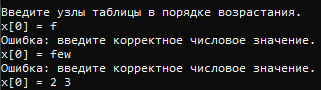
\includegraphics[scale=1]{error_2.png}
    \caption{Обработка ошибок при вводе координат точек}
    \label{fig:success}
\end{figure}

\begin{figure}[H]
    \centering
    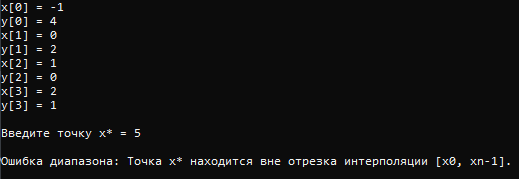
\includegraphics[scale=1]{error_3.png}
    \caption{Обработка ошибок при вводе $x^*$ вне отрезка интерполяции}
    \label{fig:success}
\end{figure}

\begin{figure}[H]
    \centering
    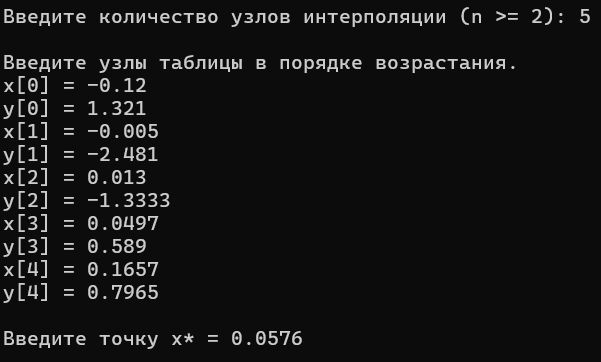
\includegraphics[scale=1]{3.png}
    \caption{Тестовый пример}
    \label{fig:success}
\end{figure}

\begin{figure}[H]
    \centering
    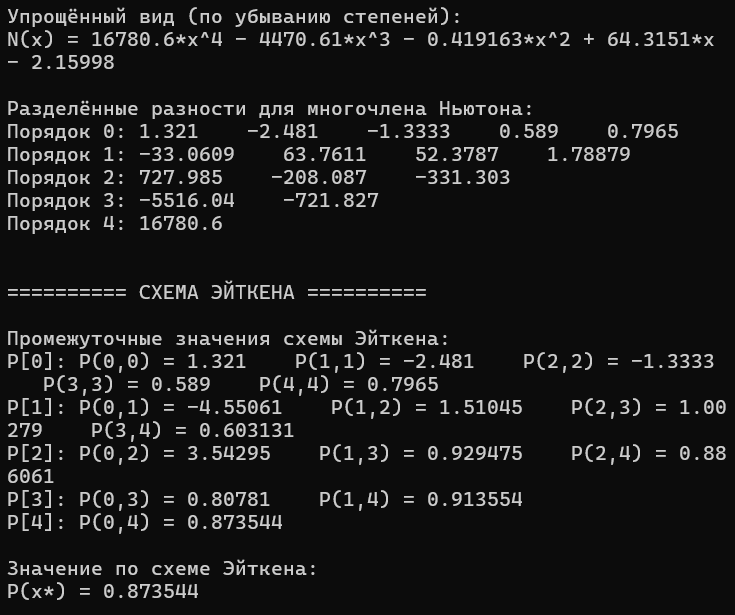
\includegraphics[scale=1]{1.png}
    \caption{Результат своей программы}
    \label{fig:success}
\end{figure}

\begin{figure}[H]
    \centering
    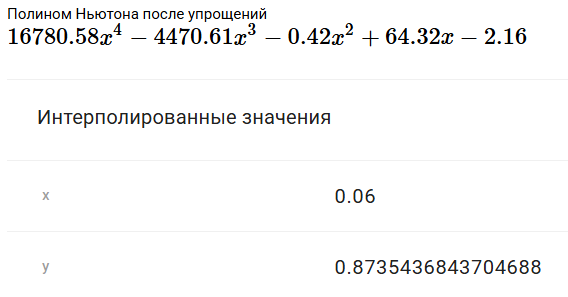
\includegraphics[scale=1]{2.png}
    \caption{Результат сторонней программы}
    \label{fig:success}
\end{figure}

\section{Вывод}

В ходе лабораторной работы была разработана программа для
интерполяции таблично заданной функции.

В программе реализовано использование трёх подходов:

\begin{itemize}
    \item интерполяционного многочлена Лагранжа;
    \item интерполяционного многочлена Ньютона;
    \item схемы Эйткена.
\end{itemize}

Для метода Ньютона была сформирована таблица разделённых
разностей, а для схемы Эйткена выведены промежуточные результаты
рекуррентных вычислений.

Кроме вычислительной части, в программе реализована обработка
некорректных входных данных: проверяется корректность числового
ввода, строгая возрастаемость узлов интерполяции и нахождение
точки $x^*$ внутри интервала интерполяции.


\end{document}